\section{Introduction}
\label{sec:intro}

Convolutional Neural Networks (CNNs) have achieved state-of-the-art results in numerous computer vision tasks, owing to their ability to learn hierarchical features and their translation equivariance. However, standard CNNs are inherently sensitive to image rotations, leading to degraded performance when processing rotated images.

%-------------------------------------------------------------------------
\subsection{Deficiencies of CNNs and the Role of Rotational Invariance}

The lack of rotational invariance in CNNs necessitates the use of data augmentation techniques, where training datasets are expanded with rotated versions of existing images. While this can improve performance, it introduces computational overhead and requires careful tuning to determine the appropriate number of rotated versions. To address this, Rotation-Invariant Convolutional Neural Networks (RIC-CNNs) \cite{mo2022riccnnrotationinvariantcoordinateconvolutional} have been proposed, utilizing rotation-invariant coordinate systems to achieve invariance to arbitrary rotations.

\subsection{Limitations of RIC-CNNs and the Need for Equivariance}

While RIC-CNNs effectively handle rotated images, their strict rotational invariance can be a limitation. In scenarios where distinguishing between rotated versions of objects is crucial (e.g., '6' vs. '9'), RIC-CNNs may struggle. In such cases, rotational equivariance – where feature maps transform in the same way as the input image – is desirable to preserve rotational information.

\subsection{Our Hybrid Approach}
To balance the strengths and weaknesses of CNNs and RIC-CNNs, we propose a hybrid approach that combines both architectures. This allows us to leverage the discriminative power of CNNs for rotation-sensitive tasks while benefiting from the robustness of RIC-CNNs to handle general image rotations. We explore several integration strategies to effectively fuse features from both networks.

%-------------------------------------------------------------------------
\subsection{Contributions}
Our contributions include:
\begin{itemize}
    \item Developing hybrid CNN-RIC-CNN architectures for improved performance on both rotated and non-rotated images.
    \item Evaluating the proposed methods on the MNIST and Traffic Signs datasets.

\end{itemize}


\section{Related Works}
\label{sec:related}

In this section, we focus on Rotation-Invariant Convolutional Neural Networks (RIC-CNNs).

\subsection{Rotation-Invariant Coordinate Convolutional Neural Network}

Mo and Zhao (2022) introduce the \emph{Rotation-Invariant Coordinate Convolution} (RIC-C) to embed structural rotation invariance into the convolution operation.  We first recall the standard convolution:

\begin{equation}
\Phi_{C}(X_0, F)
\;=\;
\sum_{P \,\in\, S} W(P)\,F(X_0 + P),
\label{eq:std_conv}
\end{equation}

\noindent
where \(S\) is the usual fixed sampling grid (e.g.\ a \(3\times3\) neighborhood) and \(W(P)\) are the kernel weights.

\begin{figure}
    \centering
    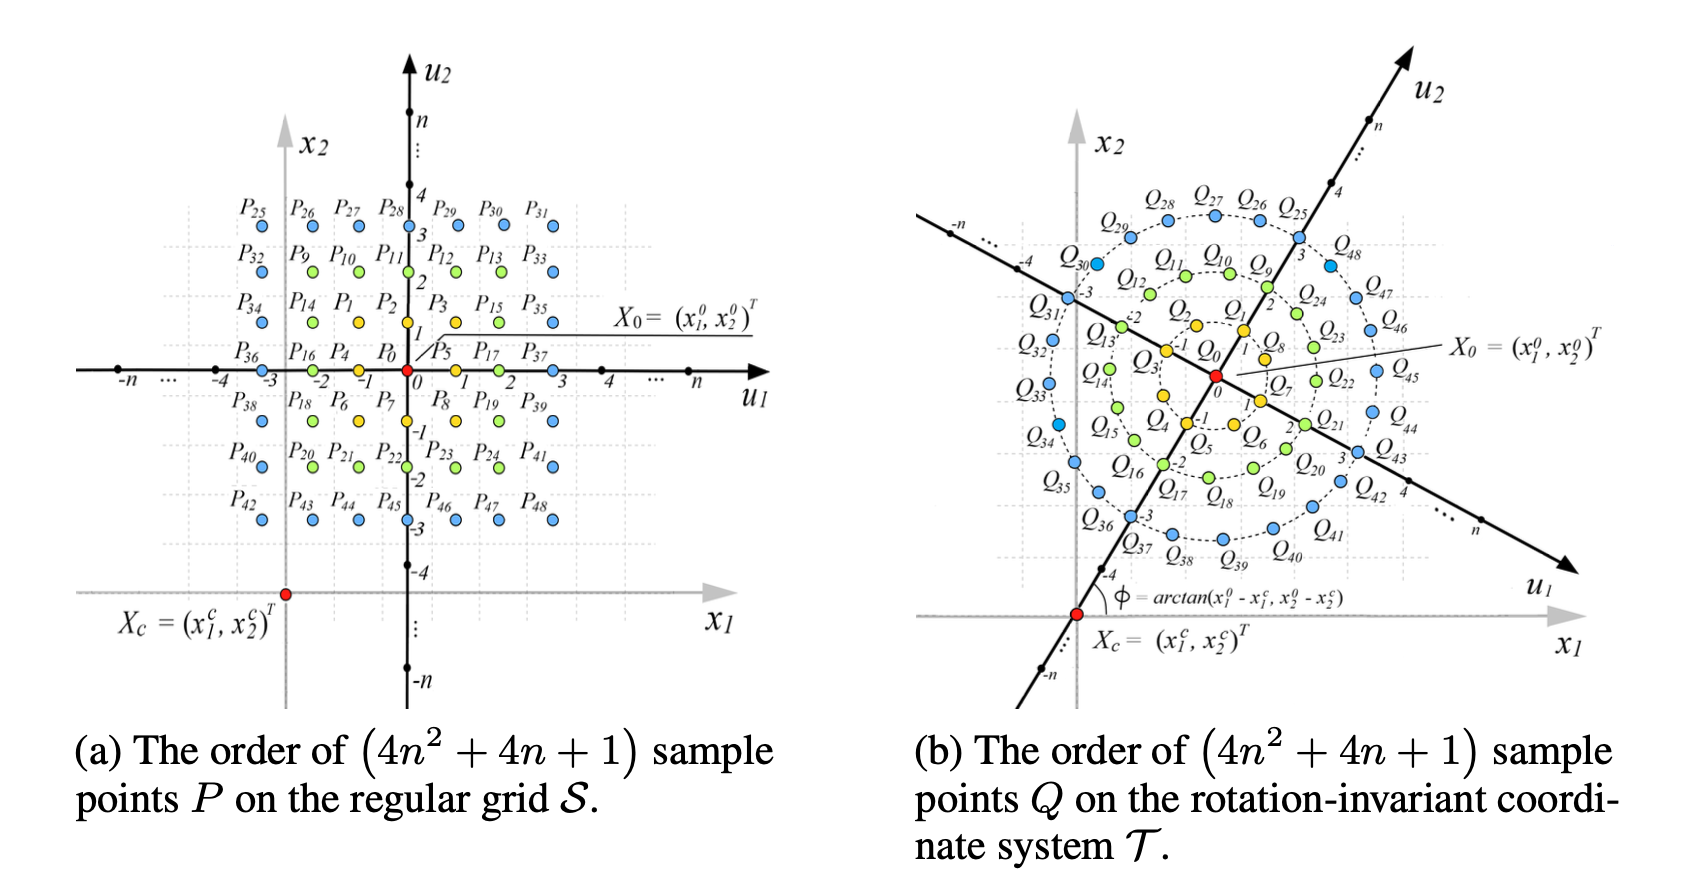
\includegraphics[width=1.0\linewidth]{author-kit-CVPR2025-v3.1-latex-/pics/ric_sample.png}
    \caption{Two sets of sampling points used for calculating $\Phi_C$ and $\Phi_{\mathrm{RIC}-C}$, respectively. It is clear that $Q_\alpha\in\mathcal T$ can be regarded as the corresponding point of $P_\alpha\in\mathcal S$, where $\alpha=0,1,2,\dots,4n^2+4n$.}
    \label{fig:ric_sample}
\end{figure}
RIC-C replaces the fixed grid \(S\) by a \emph{rotation-aware} sampling pattern \(\mathcal T_{X_0}\).  Define
\[
\varphi \;=\;atan2\bigl(x^0_2,\,x^0_1\bigr)
\quad\text{for}\quad
X_0=(x^0_1,x^0_2)^T
\]
and let the kernel cover radii \(r=1,\dots,n\).  On each circle of radius \(r\), sample
\begin{equation}
Q_{r,i}
=
\bigl(r\cos(\varphi + \tfrac{2\pi\,i}{8r}),\,r\sin(\varphi + \tfrac{2\pi\,i}{8r})\bigr),
\quad
i=0,1,\dots,8r-1.
\label{eq:ric_points}
\end{equation}
Collecting all such \(Q_{r,i}\) (plus the center \(Q_{0}=(0,0)\)) defines
\(\;\mathcal T_{X_0}=\{Q_{r,i}\}\).
The RIC-C operation is then
\begin{equation}
\Phi_{\mathrm{RIC\text{-}C}}(X_0, F)
\;=\;
\sum_{Q \,\in\, \mathcal T_{X_0}} W(Q)\,F(X_0 + Q).
\label{eq:ric_conv}
\end{equation}

\noindent
Because \(\mathcal T_{X_0}\) itself rotates by the same angle when the input is rotated about the image center, one can show
\(\Phi_{\mathrm{RIC\text{-}C}}(Y_0,G) = \Phi_{\mathrm{RIC\text{-}C}}(X_0,F)\)
for any rotation \(G(Y) = F(R_{-\theta} Y)\), proving invariance. In \ref{fig:ric_sample}, the sampling scheme of each method can be compared.

\subsubsection*{Key Limitations}

\begin{itemize}
  \item \textbf{Loss of Orientation Information.}  Enforcing full invariance discards absolute angle cues, making it hard to distinguish classes that differ only by rotation (e.g.\ ‘6’ vs.\ ‘9’).  
  \item \textbf{Center-Only Invariance.}  The proof assumes rotations about the image (or feature-map) center; arbitrary pivot points are not covered.  
  \item \textbf{Interpolation \& Pooling Artifacts.}  Sampling at fractional coordinates requires interpolation (e.g.\ bilinear), and subsequent max-pooling layers are not strictly equivariant, leading to small but accumulative errors.
\end{itemize}